\documentclass[a4paper,11pt]{article}
\usepackage[utf8]{inputenc}
\usepackage[T1]{fontenc}
\usepackage[french]{babel}
\usepackage{textcomp}
\usepackage{listings}
\usepackage{pdfpages}
\usepackage{array}
\usepackage{fullpage}

\title{PROJET\\ UE Méthodes de ranking et recommandations\\ 
		Sujet 5 : Simulation d'un Google Bombing}
\author{Maxime Gonthier - Laureline Martin}

\begin{document}

\pagenumbering{gobble}\clearpage
	\pagenumbering{gobble}\clearpage
	\maketitle
	\newpage\clearpage\pagenumbering{arabic}

\newpage
\tableofcontents
\newpage

\section{Introduction}
	
	
\section{Manuel utilisateur}

\section{Plan}
	Dans un premier temps nous allons effectué des tests simples en utilisant quatre type de structures différentes ainsi que trois cibles de pertinences différentes.
	Nous en déduirons des hypothèses sur l'eficacité de chaque structure et l'impact de la pertinence de la cible sur cette même efficacité.
	Dans un second temps nous étudierons l'impact sur la pertinence de graphes générés en nombre aléatoire pour étudier qu'elle structure est globalement la plus efficace.
	Puis nous testerons la meme choses avec cette fois ci un graphe dont les arcs le reliant a lui meme sont générées aléatoirement.
	Enfin nous ferons varier le nombre de sommets du graphe ataquant pour en déduire son efficacité et nous conclurons.
	
\section{I.		Expériences initiales et hypothèses}
	
	L'algorithme power calculant les pertinences est contenu dans le fichier $ranking.c$. Il n'est pas détaillé dans ce rapport mais le fichier est commenté.
	On considère ici le graphe du web Stanford.txt. Ce graphe est modifié par l'ajout de sommets et d'arcs afin d'augmenter la valeur d'un sommet ciblé.\\
	On considère que :\\
	\begin{itemize}
		\item Les sommets représentent les pages du web.
		\item Les arcs représentent les liens dirigeant vers d'autres pages.
		\item Les valeurs des sommets représentent les pertinences calculés par l'algorithme pagerank.
		\item Le sommet cible représente la page dont on souhaite augmenter la pertinence.
		\item 100 sommets sont ajoutés pour chaque test.
	\end{itemize}
	\subsection{Explication du code}
	\subsection{Résultats des tests initiaux}
		\subsubsection{Stanford.txt sans modification}
			281903 pages\\
			2312497 liens\\
			132 itérations\\
			27.627466 secondes\\
			\\
			Voici les pertinences de base des trois sommets étudiés :\\
			Pertinence forte : Page 280545 - 9.96199e-05\\
			Pertinence moyenne : Page 281466 - 7.53954e-06\\
			Pertinence faible : Page 281574 - 6.05222e-07\\
			\\
		\subsubsection{Résultats}
			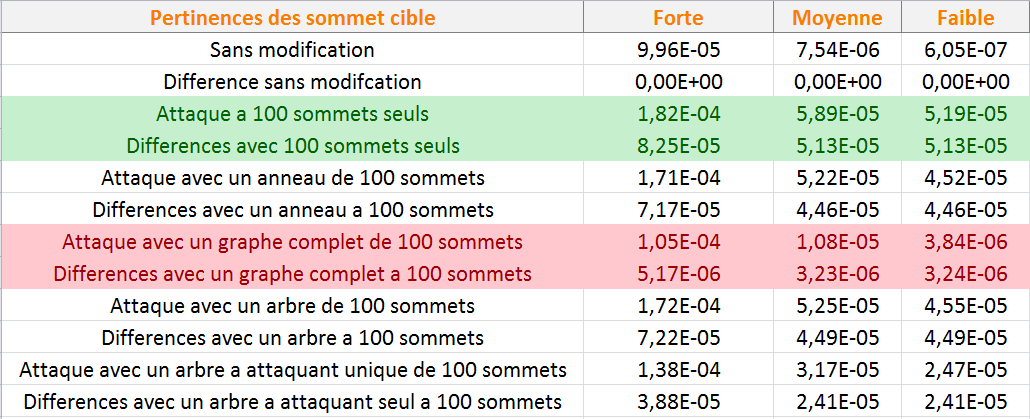
\includegraphics[scale = 0.5]{Captures/ranking1.PNG}
		\subsubsection{Analyses}
			
		\subsubsection{Hypothèses}
			
	\subsection{Conclusion des tests initiaux et hypothèses}
		

\section{II.	Expériences avec un nombre de graphes générés aléatoirement}
	Nous allons désormais insérer des graphes générés aléatoirement. Ce qui est aléatoire n'est pas la structure des graphes mais le nombre de garphes générés.
	L'objectif de cette démarche est de déterminer quel structure est la plus efficace globalement.
	C'est a dire quelle structure influe le plus sur la pertinence quelle que soit la situation.
	De plus les resultats nous aiderons aussi a determiner l'impact qu'a une certaine structure sur la cible de manière plus générale 
	que dans les cas prédéfinis de la partie précedente.
	Le nombre de sommet des graphes ajoutées est fixé a 100.
	La cible est également fixé ainsi que la structure des graphes ajoutées.
	On va par exemple insérez 5 graphes complet de nombre de sommet respectivement : 25, 10, 5, 6 et 4. Tous reliées au sommet cible.
	Dans un premier temps nous allons expliquer le code derrière cette démarche puis nous analyserons les résultats.
	\subsection{Explication du code}
		Tous est dans le fichier $ajoutsommetsattanquants.c$. Les fonctions utilisées sont $ajoutanneaualeatoire$, $ajoutcompletaleatoire$
		et $ajoutarbrealeatoire$. Ces fonctions reprennent en partie le code des trois fonctions presque eponyme décrite précedemment.
		Regardons ce qui a changé. 
		\begin{lstlisting}
	while(nbsommetrestant > 0) {
		nbajout = rand()%(100-nouveausommets);
		if (nbajout <= 3) { nbajout = 3; }
		nbsommetrestant -= nbajout;
		\end{lstlisting}
		$nbajout$ représente le nombre de sommet que l'on va ajouter dans la première structure créer. Il choisis donc un nombre 
		aléatoire entre 0 et 100 car le nombre de sommet total est limité a 100. Si le nombre choisis est inférieur a 3 on le fixe a 3 car créer
		des anneau ou des graphes complets de tailles inférieure a 3 reviens juste a créer des sommets seuls.
		$nbajout$ est enlevé au nombre de sommet restant a ajouter. Puis on lance la construction de la structure comme vu précedemment 
		avec $nbajout$ représentant le nombre de sommets. A la fin de cette itération $nbajout$ reprends un nombre aléatoire qui cette fois
		prend une valeur entre 0 et 100 moins le nombre de sommets ajouté precedement représenté par $nouveausommets$.
	\subsection{Résultats des tests}
		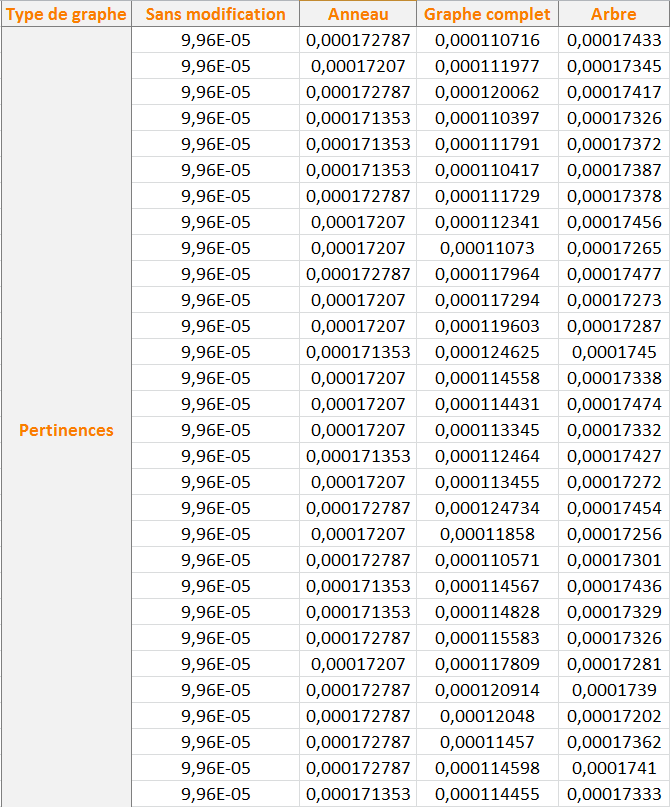
\includegraphics[scale = 0.5]{Captures/ranking2.PNG}\\
		ANALYSE\\
		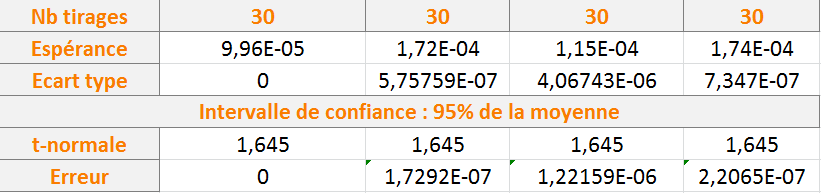
\includegraphics[scale = 0.5]{Captures/ranking3.PNG}\\
		ANALYSE\\

	\subsection{Analyse graphes en anneau}
		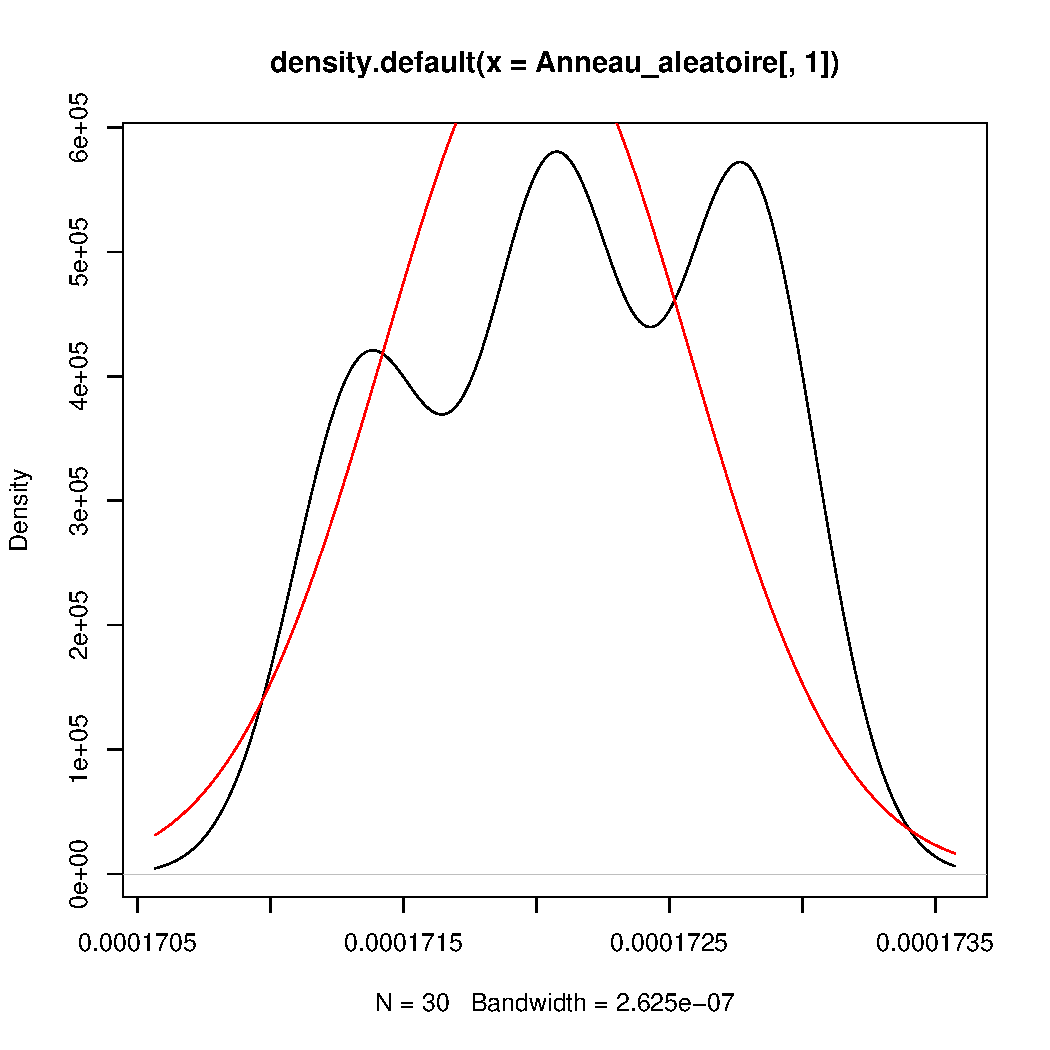
\includepdf{../R/Nombre_de_graphe_aleatoire/Anneau.pdf}
	\subsection{Analyses Graphes complet}
		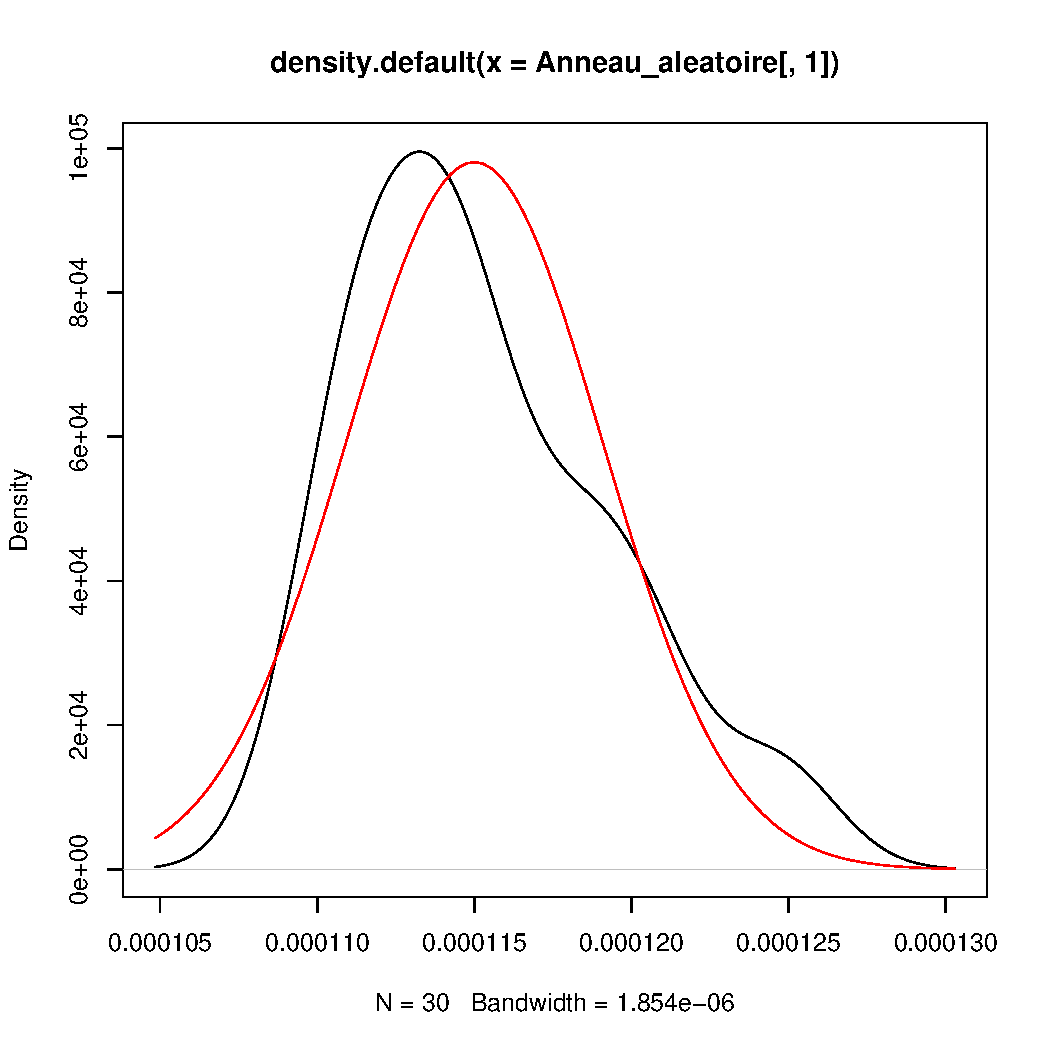
\includepdf{../R/Nombre_de_graphe_aleatoire/Complet.pdf}
	\subsection{Analyses Arbres}
		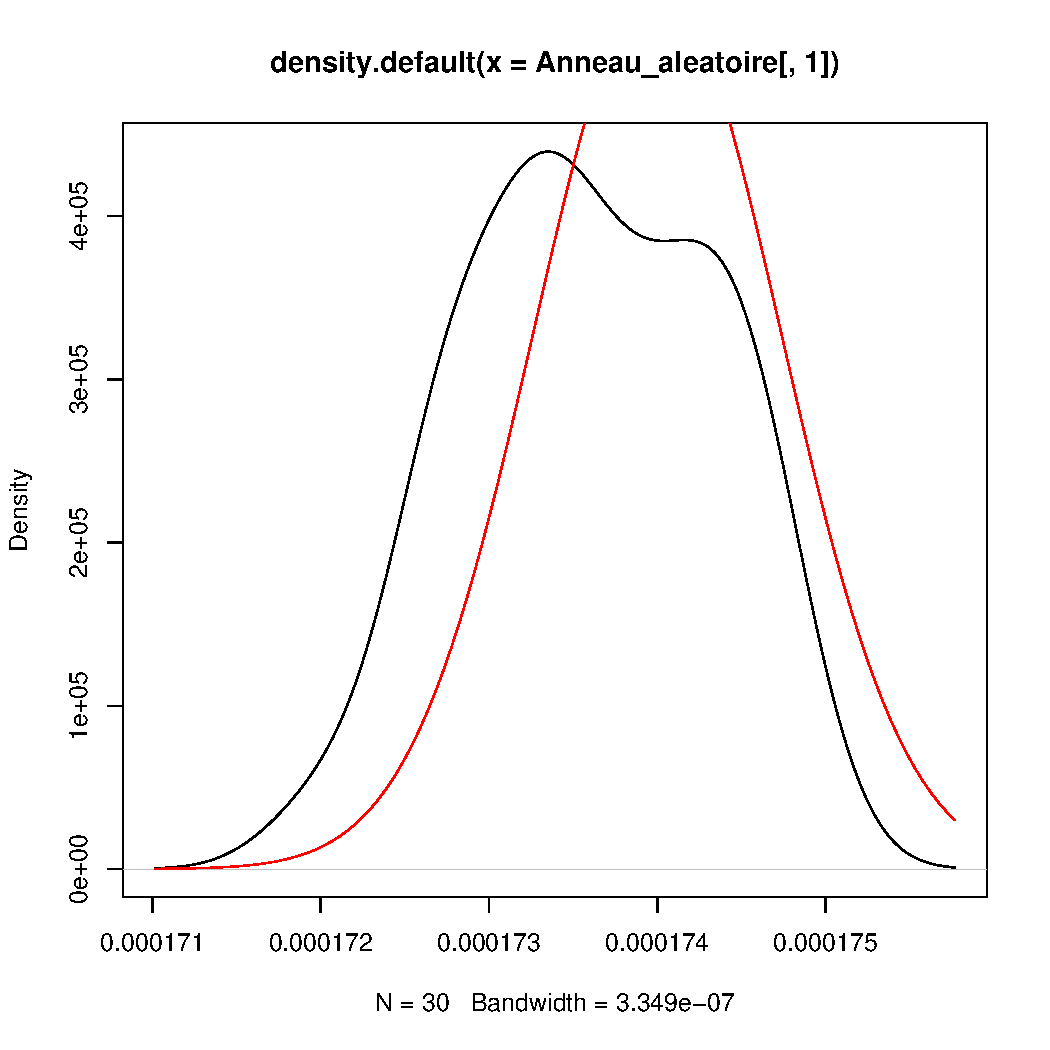
\includepdf{../R/Nombre_de_graphe_aleatoire/Arbre.pdf}
	\subsection{Conclusion sur l'impact de chaque structure}

\section{III.	Expériences avec un graphe de degré aléatoire}
	\subsection{Résultats des tests}
		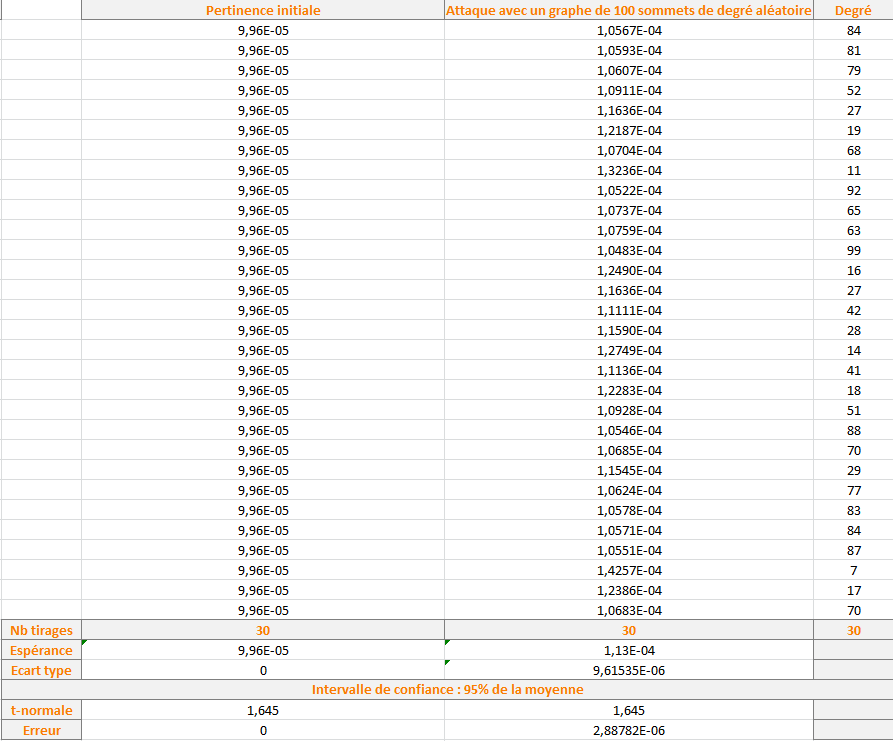
\includegraphics[scale = 0.5]{Captures/ranking4.PNG}\\
	\subsection{Analyses}
	
\section{IV.	Expériences sur l'efficacité}
	\subsection{Résultats des tests}
		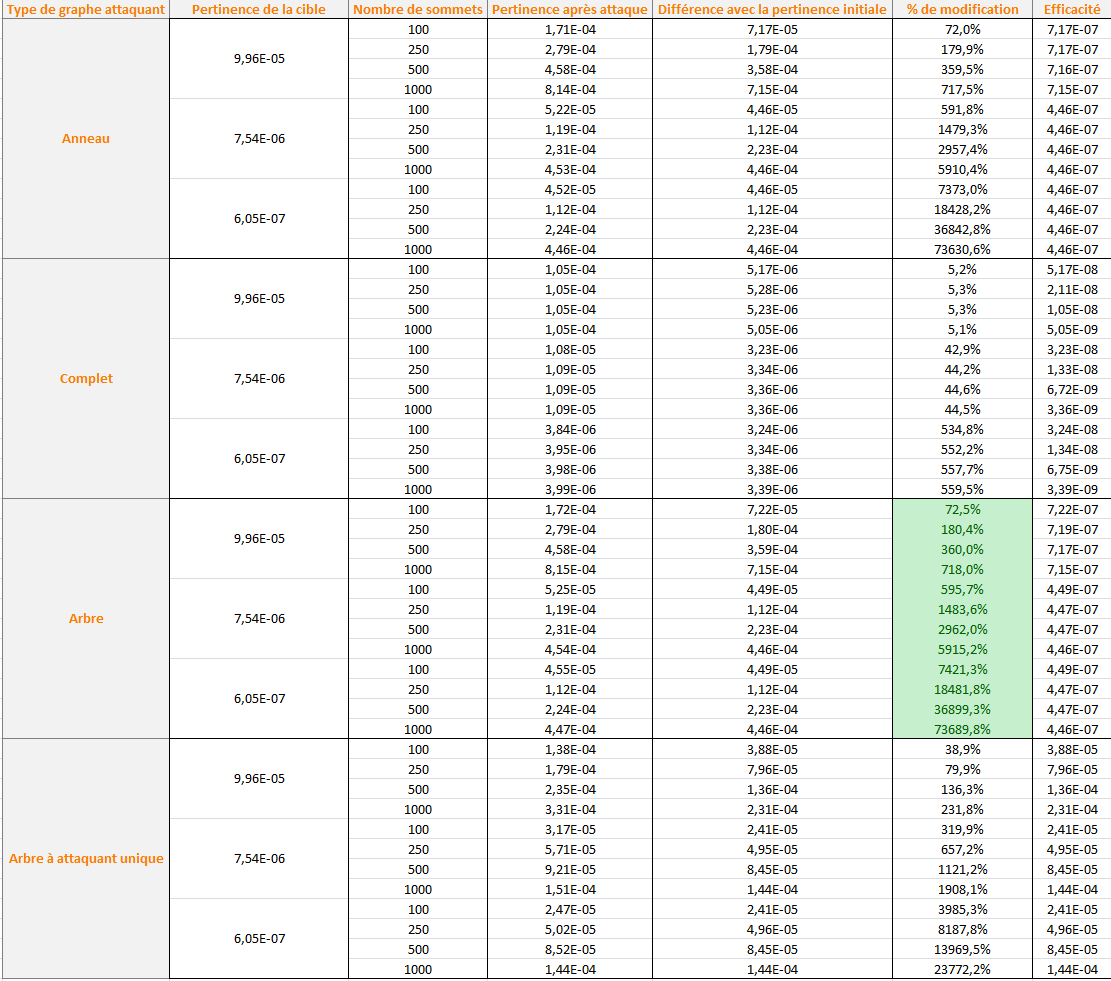
\includegraphics[scale = 0.6]{Captures/ranking5.PNG}\\
	\subsection{Analyses}
	
\section{V.		Conclusion}

\end{document}
